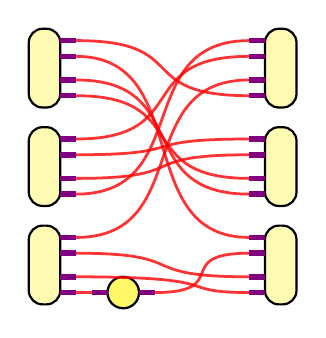
\begin{tikzpicture}


%vertex for $ a_q^* a_q $
\filldraw[fill = yellow!60!white, thick] (-0.5,-0.1) circle (0.2);

%vertices for $ B_4 $ - right
\filldraw[thick, rounded corners = 5, fill = yellow!30!white] (-1.7,-0.25) rectangle ++(0.4,1);
\filldraw[thick, rounded corners = 5, fill = yellow!30!white] (-1.7,1) rectangle ++(0.4,1);
\filldraw[thick, rounded corners = 5, fill = yellow!30!white] (-1.7,2.25) rectangle ++(0.4,1);

%vertices for $ B_4 $ - left
\filldraw[thick, rounded corners = 5, fill = yellow!30!white] (1.3,-0.25) rectangle ++(0.4,1);
\filldraw[thick, rounded corners = 5, fill = yellow!30!white] (1.3,1) rectangle ++(0.4,1);
\filldraw[thick, rounded corners = 5, fill = yellow!30!white] (1.3,2.25) rectangle ++(0.4,1);

%connectors
\draw[line width = 2, red!50!blue] (-0.7,-0.1) -- ++(-0.2,0);
\draw[line width = 2, red!50!blue] (-0.3,-0.1) -- ++(0.2,0);

\draw[line width = 2, red!50!blue] (-1.1,-0.1) -- ++(-0.2,0);
\draw[line width = 2, red!50!blue] (-1.1,0.1) -- ++(-0.2,0);
\draw[line width = 2, red!50!blue] (-1.1,0.4) -- ++(-0.2,0);
\draw[line width = 2, red!50!blue] (-1.1,0.6) -- ++(-0.2,0);

\draw[line width = 2, red!50!blue] (-1.1,1.15) -- ++(-0.2,0);
\draw[line width = 2, red!50!blue] (-1.1,1.35) -- ++(-0.2,0);
\draw[line width = 2, red!50!blue] (-1.1,1.65) -- ++(-0.2,0);
\draw[line width = 2, red!50!blue] (-1.1,1.85) -- ++(-0.2,0);

\draw[line width = 2, red!50!blue] (-1.1,2.4) -- ++(-0.2,0);
\draw[line width = 2, red!50!blue] (-1.1,2.6) -- ++(-0.2,0);
\draw[line width = 2, red!50!blue] (-1.1,2.9) -- ++(-0.2,0);
\draw[line width = 2, red!50!blue] (-1.1,3.1) -- ++(-0.2,0);

\draw[line width = 2, red!50!blue] (1.1,-0.1) -- ++(0.2,0);
\draw[line width = 2, red!50!blue] (1.1,0.1) -- ++(0.2,0);
\draw[line width = 2, red!50!blue] (1.1,0.4) -- ++(0.2,0);
\draw[line width = 2, red!50!blue] (1.1,0.6) -- ++(0.2,0);

\draw[line width = 2, red!50!blue] (1.1,1.15) -- ++(0.2,0);
\draw[line width = 2, red!50!blue] (1.1,1.35) -- ++(0.2,0);
\draw[line width = 2, red!50!blue] (1.1,1.65) -- ++(0.2,0);
\draw[line width = 2, red!50!blue] (1.1,1.85) -- ++(0.2,0);

\draw[line width = 2, red!50!blue] (1.1,2.4) -- ++(0.2,0);
\draw[line width = 2, red!50!blue] (1.1,2.6) -- ++(0.2,0);
\draw[line width = 2, red!50!blue] (1.1,2.9) -- ++(0.2,0);
\draw[line width = 2, red!50!blue] (1.1,3.1) -- ++(0.2,0);


%first loop
\draw[red, opacity = .8, line width = 1] (-1.1,-0.1) -- (-0.9,-0.1);
\draw[red, opacity = .8, line width = 1] (-1.1,0.1) .. controls ++(2,0) and ++(-1,0) .. (1.1,-0.1);
\draw[red, opacity = .8, line width = 1] (1.1,0.1) .. controls ++(-1.5,0) and ++(1.5,0) .. (-1.1,0.4);
\draw[red, opacity = .8, line width = 1] (-1.1,0.6) .. controls ++(1.5,0) and ++(-1.5,0) .. (1.1,2.6);
\draw[red, opacity = .8, line width = 1] (1.1,2.4) .. controls ++(-1.5,0) and ++(1.5,0) .. (-1.1,3.1);
\draw[red, opacity = .8, line width = 1] (-1.1,2.9) .. controls ++(1.5,0) and ++(-1.5,0) .. (1.1,0.6);
\draw[red, opacity = .8, line width = 1] (1.1,0.4) .. controls ++(-1,0) and ++(1,0) .. (-0.1,-0.1);


%second loop
\draw[red, opacity = .8, line width = 1] (-1.1,1.35) .. controls ++(1.5,0) and ++(-1.5,0) .. (1.1,1.65);
\draw[red, opacity = .8, line width = 1] (1.1,1.85) .. controls ++(-1.5,0) and ++(1.5,0) .. (-1.1,1.65);
\draw[red, opacity = .8, line width = 1] (-1.1,1.85) .. controls ++(1.5,0) and ++(-1.5,0) .. (1.1,2.9);
\draw[red, opacity = .8, line width = 1] (1.1,3.1) .. controls ++(-1.5,0) and ++(1.5,0) .. (-1.1,1.15);


%third loop
\draw[red, opacity = .8, line width = 1] (-1.1,2.6) .. controls ++(1.5,0) and ++(-1.5,0) .. (1.1,1.15);
\draw[red, opacity = .8, line width = 1] (1.1,1.35) .. controls ++(-1.5,0) and ++(1.5,0) .. (-1.1,2.4);


\end{tikzpicture}